\documentclass[parskip=full]{scrartcl}

\usepackage[utf8]{inputenc} % use utf8 file encoding for TeX sources
\usepackage[T1]{fontenc} % avoid garbled Unicode text in pdf
\usepackage[german]{babel} % german hyphenation, quotes, etc
\usepackage{hyperref} % detailed hyperlink/pdf configuration
\hypersetup{ % ‘texdoc hyperref‘ for options
pdftitle={Lamb.da - Das Spiel}
}
\usepackage{csquotes} % provides \enquote{} macro for "quotes"
\usepackage{graphicx}

\usepackage{enumerate}

\begin{document}

\title{Lamb.da - Das Spiel}
%\date{October 12, 123}
\author{Name, Name, Name}
\maketitle

\input{./sections/1_introduction.tex}
\input{./sections/2_target_definition.tex}
\input{./sections/3_product_application.tex}
\input{./sections/4_product_environment.tex}
\section{Funktionale Anforderungen}

\begin{itemize}
\item \textbackslash F10 \textbackslash Anforderungsbeschreibung
\end{itemize}
\section{Produktdaten}

\begin{itemize}
\item \textbackslash D10 \textbackslash Beschreibung des Subjekts, über welches Daten gespeichert werden
\begin{itemize}
\item \textbackslash LD10 \textbackslash Beschreibung der Daten, die zum Subjekt gespeichert werden
\end{itemize}
\end{itemize}
\section{Nichtfunktionale Anforderungen}

\begin{itemize}
\item /NF10/ Anforderungsbeschreibung
\end{itemize}
\section{Systemmodelle}

\subsection{Globale Testfälle}
Folgende Funktionssequenzen sind zu überprüfen:

\begin{itemize}
\item \textbackslash T10 \textbackslash Funktionssequenzbeschreibung
\end{itemize}

\subsection{Datenkonsistenzen}

\begin{itemize}
\item \textbackslash T30 \textbackslash Datenkonsistenzbeschreibung
\end{itemize}

\subsection{Objektmodell}
% UML Klassendiagramme

\begin{figure}[h]
\centering
\includegraphics[scale=0.35]{../system_models/object_models/lambda_calculus.pdf}
\caption{UML Klassendiagramm zum Lambda-Kalkül}
\end{figure}

\subsection{Dynamische Modelle}
% UML Zustandsautomat, Sequenzdiagramm

\begin{figure}[h]
\centering
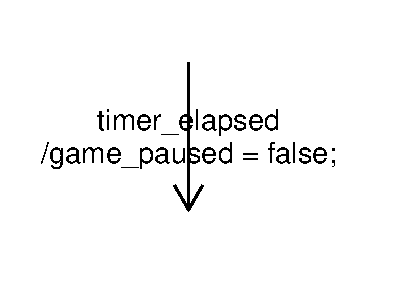
\includegraphics[scale=0.3]{../system_models/dynamic_models/menu_state_machine.pdf}
\caption{Zustandsautomat zur Menübedienung}
\end{figure}

\begin{figure}[h]
\centering
\includegraphics[scale=0.6]{../system_models/dynamic_models/game_level_state_machine.pdf}
\caption{Zustandsautomat zum Ablauf eines Levels}
\end{figure}

\begin{figure}[h]
\centering
\includegraphics[scale=0.6]{../system_models/dynamic_models/reduction_mode_state_machine.pdf}
\caption{Zustandsautomat zur Funktion des Reduktions-Modus}
\end{figure}

\subsection{Benutzerschnittstelle}

GUI
\input{./sections/9_glossary.tex}

\end{document}